The user interface is made as a windows form application\footnote{graphical application programming interface, included in the .NET Framework.}. Using Visual Studios designer tools, it is simple to make a graphical user interface with buttons, panels, and windows just the way you want.\\
   The main idea of the design of the user interface is that it should be intuitive, which  the user should not spend a lot of time figuring out what all the buttons do. Furthermore we have designed the interface so the main structure looks like other popular strategy computer games (see \ref{pic:red_alert} and \ref{pic:coc} in appendix). We have done this to make the application easy to learn how to use.
	
\subsection*{Game Start Settings}
When the game is started, a dialog box is shown where one can choose the size of the \textit{war zone}. We have chosen to have three fixed grid sizes, because of the way we draw the grid \ref{sec:drawing}.\\
   The functions of the dialog box is:
\begin{enumerate}
	\item \textit{Small, Medium, Large} radio buttons - select one to choose the grid size.
	\item \textit{Start} button - starts the game.
\end{enumerate}

\begin{figure}[H]
\begin{center}
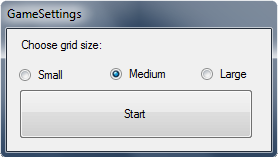
\includegraphics[scale=0.9]{Images/dialog.png}
\end{center}
\caption{Screen shot of the game settings dialog box.}
\label{dialog}
\end{figure}

\subsection*{Game Interface Functions}
The functions of the game interface is:
\begin{enumerate}
	\item \textit{War zone} - contains the grid on which the war game unfolds.
	\item \textit{Agents} - the agents of the different teams (here with a 4-player game setup).
	\item \textit{Command center} - here the user types the commands to navigate the agents around the grid.
	\item \textit{Stats field} - shows the stats of a selected agent.
	\item \textit{Agents left} - shows how many agents are left on the teams.
	\item \textit{Combat log} - contains a combat log on who killed who in fights between agents.
	\item \textit{Command list} - contains the list of available commands the user can type in the \textit{command center}.
	\item \textit{MousePos grid} - shows the grid point of the mouse position.
	\item \textit{Execute} button - executes the typed in command in the \textit{command center}.
	\item \textit{End turn} button - ends the turn and gives the turn to the next player.
	\item \textit{Reset game} button - sets up a new game.
	\item \textit{Quit game} button - closes the game.
\end{enumerate}

\begin{figure}[H]
\begin{center}
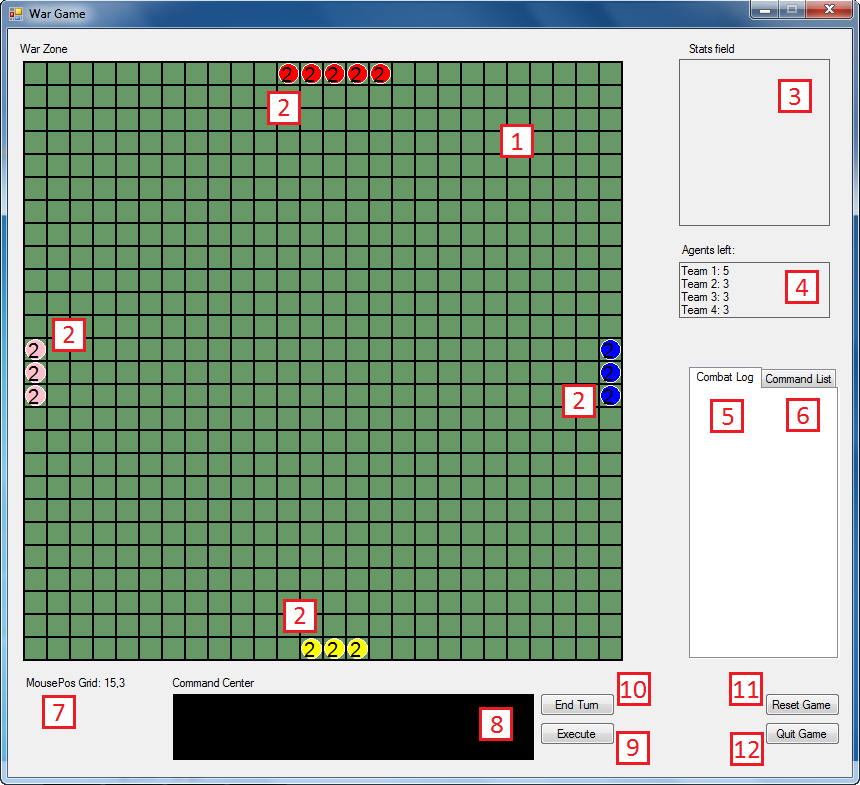
\includegraphics[scale=0.6]{Images/game_interface.png}
\end{center}
\caption{Screen shot of the game interface.}
\label{game_interface}
\end{figure}

\subsection*{Drawing the Grid and Agents}
\label{sec:drawing}
The program make use of GDI+ \cite{misc:gdiplus} to draw the grid (the war zone) on the screen. A usercontrol is added to eliminate the flickering GDI+ normally creates on windows forms, this is done with the help of double buffering.
We only use GDI+ graphics inside the usercontrol DBpanel, and make sure we draw things in the correct order, as we draw the pixels untop of each other. The first thing drawn is the background, which in our case is green, with the black gridlines on top of it, to create the game grid. Next the agents are drawn, one after the another.
The agent's start posistions are calculated by the following algorithm:
\begin{source}{This code snippet calculates the agent's start positions}{}                 
            int it1 = (Grids / 2) - (agentsOnTeam1 / 2);
            int it2 = (Grids / 2) - (agentsOnTeam2 / 2);
            int it3 = (Grids / 2) - (agentsOnTeam3 / 2);
            int it4 = (Grids / 2) - (agentsOnTeam4 / 2);
            foreach (Agent a in agents)
            {
                Point p = new Point();
                if (a.team.ID == 1)
                {
                    p = getGridPixelFromGrid(new Point(it1, 0));
                }
                else if (a.team.ID == 2)
                {
                    p = getGridPixelFromGrid(new Point(Grids - 1, it2));
                }
                else if (a.team.ID == 3)
                {
                    p = getGridPixelFromGrid(new Point(it3, Grids - 1));
                }
                else if (a.team.ID == 4)
                {
                    p = getGridPixelFromGrid(new Point(0, it4));
                }

                a.posX += p.X;
                a.posY += p.Y;

                if (a.team.ID == 1)
                {
                    it1++;
                }
                else if (a.team.ID == 2)
                {
                    it2++;
                }
                else if (a.team.ID == 3)
                {
                    it3++;
                }
                else if (a.team.ID == 4)
                {
                    it4++;
                }
            }
\end{source}
It is the start location for each team. If the grid is 13 "grids" wide and team one consists of three agents, the starting position for team one will be (13/2) - (3 / 2) = 6,5 - 1,5 = 5.